%To compile as handout, use
%pdflatex "\def\ishandout{1} \input{filename.tex}"
%Defaults to non-handout mode (with slide reveals)
\ifdefined\ishandout
  \documentclass[handout]{beamer}
\else
  \documentclass{beamer}
\fi
 
\usepackage{econ103slides} 

\date{Lecture \# 5}
\begin{document} 



%%%%%%%%%%%%%%%%%%%%%%%%%%%%%%%%%%%%%%%%

\begin{frame}[plain]
	\titlepage 
	

\end{frame} 
%%%%%%%%%%%%%%%%%%%%%%%%%%%%%%%%%%%%%%%%
\begin{frame}

\begin{center}
 \Huge Basic Probability -- Part I
\end{center}

\end{frame}
%%%%%%%%%%%%%%%%%%%%%%%%%%%%%%%%%%%%%%%%%
%\begin{frame}
%
%\centering \Huge How Good are Your Intutions?\\
%\normalsize ``Seven Odd Questions'' \href{http://www.amazon.com/An-Introduction-Probability-Inductive-Logic/dp/0521775019/ref=cm_cr_pr_product_top}{\fbox{Hacking, 2001}}
%
%\end{frame}
%
%%%%%%%%%%%%%%%%%%%%%%%%%%%%%%%%%%%%%%%%%
%
%
%
%\begin{singlespace}
%%%%%%%%%%%%%%%%%%%%%%%%%%%%%%%%%%%%%%%%%
%\begin{frame}
%\frametitle{``Odd Question'' \# 1}
%
%About as many boys as girls are born in hospitals. Many babies are born every week at City General. In Cornwall, a country town, there is a small hospital where only a few babies are born every week. A \emph{normal} week is one where between 45\% and 55\% of babies are females. An \emph{unusual} week is one where more than 55\% are girls, or more than 55\% are boys. 
%
%	\vspace{1em}
%	Which of the following is true:
%		\begin{enumerate}[(a)]
%			\item Unusual weeks occur equally often at City General and at Cornwall.
%			\item Unusual weeks are more common at City General.
%			\item Unusual weeks are more common at Cornwall.
%		\end{enumerate}
%\end{frame}
%%%%%%%%%%%%%%%%%%%%%%%%%%%%%%%%%%%%%%%%%
%\begin{frame}
%\frametitle{``Odd Question'' \# 2}
%Pia is thirty-one years old, single, outspoken, and smart. She was a philosophy major. When a student, she was an ardent supporter of Native American rights, and she picketed a department store that had no facilities for nursing mothers. 
%
%\vspace{1em}
%Rank the following statements in order from most probable to least probable.
%		\begin{enumerate}[(a)]
%			\item Pia is an active feminist.
%			\item Pia is a bank teller.
%			\item Pia works in a small bookstore.
%			\item Pia is a bank teller and an active feminist.
%			\item Pia is a bank teller and an active feminist who takes yoga classes.
%			\item Pia works in a small bookstore and is an active feminist who takes yoga classes.
%		\end{enumerate}
%\end{frame}
%%%%%%%%%%%%%%%%%%%%%%%%%%%%%%%%%%%%%%%%%
%\begin{frame}
%\frametitle{``Odd Question'' \# 3}
%In Lotto 6/49, a standard government-run lottery, you choose 6 out of 49 numbers (1 through 49). You win the biggest prize--maybe millions of dollars--if these 6 are drawn. (The prize money is divided between all those who choose the lucky numbers. If no one wins, then most of the prize money is put back into next weeks lottery.)
%	
%	Suppose your aunt offers you, \emph{free}, a choice between two ticket in the lottery, with numbers as shown:
%		\begin{enumerate}[I.]
%			\item You win if 1,2,3,4,5, and 6 are drawn.
%			\item You win if 39, 36, 32, 21, 14, and 3 are drawn.
%		\end{enumerate}
%		\vspace{1em}
%		Do you prefer I, II, or are you indifferent between the two?
%		\begin{enumerate}[(a)]
%			\item Prefer I
%			\item Prefer II
%			\item Indifferent
%		\end{enumerate}
%\end{frame}
%%%%%%%%%%%%%%%%%%%%%%%%%%%%%%%%%%%%%%%%%
%\begin{frame}
%\frametitle{``Odd Question'' \# 4}
%To throw a total of 7 with a pair of dice, you have to get a 1 and a 6, or a 2 and a 5, or a 3 and a 4.
%To throw a total of 6 with a pair of dice, you have to get a 1 and a 5, or a 2 and a 4, or a 3 and another 3.
%	\vspace{1em}
%	With two fair dice, you would expect:
%		\begin{enumerate}[(a)]
%			\item To throw 7 more frequently than 6.
%			\item To throw six more frequently than 7.
%			\item To throw 6 and 7 equally often.
%		\end{enumerate}
%\end{frame}
%%%%%%%%%%%%%%%%%%%%%%%%%%%%%%%%%%%%%%%%%
%\begin{frame}
%\frametitle{``Odd Question'' \# 5}
%\small
%You have been called to jury duty in a town where there are two taxi companies, Green Cab Ltd.\ and Blue Taxi Inc. Blue taxi uses cars painted blue; Green Cabs uses green cars. Green cabs dominates the market, with 85\% of the taxis on the road. On a misty winter night a taxi sideswiped another car and drove off. A witness says it was a blue cab. The witness is tested under conditions like those on the night of the accident, and 80\% of the time she correctly reports the color of the cab that is seen. That is, regardless of whether she is shown a blue or a green cab in misty evening light, she gets the color right 80\% of the time.
%	\vspace{1em}
%	
%	You conclude, on the basis of this information:
%		\begin{enumerate}[(a)]
%			\item The probability that the sideswiper was blue is 0.8.
%			\item It is more likely that the sideswiper was blue, but the probability is less than 0.8. 
%			\item It is just as probable that the sideswiper was green as that it was blue. 
%			\item It is more likely than not that the sideswiper was green.
%		\end{enumerate}
%\end{frame}
%
%%%%%%%%%%%%%%%%%%%%%%%%%%%%%%%%%%%%%%%%%
%\begin{frame}
%\frametitle{``Odd Question'' \# 6}
%\small
%You are a physician. You think it is quite likely that one of your patients has strep throat, but you aren't sure. You take some swabs from the throat and send them to a lab for testing. The test is (like nearly all lab tests) not perfect. 
%	\begin{itemize}
%		\item If the patient has strep throat, then 70\% if the time the lab says yes. But 30\% of the time it says NO.
%		\item If the patient does not have strep throat, then 90\% of the time the lab says NO. But 10\% of the time it says YES.
%	\end{itemize}
%	You send five successive swabs to the lab, from the same patient. and get back these results in order: YES, NO, YES, NO, YES. You conclude:
%		\begin{enumerate}[(a)]
%			\item These results are worthless.
%			\item It is likely that the patient does not have strep throat.
%			\item It is slightly more likely than not, that the patient does have strep throat.
%			\item It is very much more likely than not, that the patient does have strep throat.
%		\end{enumerate}
%\end{frame}
%
%
%\end{singlespace}
%%%%%%%%%%%%%%%%%%%%%%%%%%%%%%%%%%%%%%%%
\begin{frame}
\frametitle{``Odd Question'' \# 7}
\normalsize
`Imitate'' a coin. That is, write down a sequence of 100 H (for heads) and T (for tails) without tossing a coin--but a sequence that you think will fool everyone into thinking it is the reporting of tossing a fair coin.
		
\end{frame}

%%%%%%%%%%%%%%%%%%%%%%%%%%%%%%%%%%%%%%%%
\begin{frame}[fragile]
\frametitle{Which of these is a real sequence of coin flips? \hfill 
\includegraphics[scale = 0.05]{./images/clicker}}
\small
\begin{block}{Exhibit A}
H H H H T H H T T T H H T T T H T T T H T T H H T \\
T T T H T T T H T H T T H H H H T T T T T H H H H \\
H T T H T T H H T T H H H H H T H H T H T H T H T \\
T H H T H H T T T H T T T T T T T T T H H T T T T 
\end{block}

\begin{block}{Exhibit B}
H H T H T T T H H T H H H T H T T T H T H H T T T\\
T H H T T T H H H T H T T T H T T H H T H H T H T\\
T T H H H T H T T H T H H T	T H H H T H T T H H H\\
T T H H H H T H T T H H T T T H H T H H H T T H T
\end{block}
\end{frame}
%%%%%%%%%%%%%%%%%%%%%%%%%%%%%%%%%%%%%%%%
\begin{frame}
\frametitle{How could we tell which are the real coin flips?}
\framesubtitle{Hacking (2001, p.\ 31)}
	\begin{quote}
    Hardly anyone making up a sequence of 10 tosses puts in a run of 7 heads in a row. It is true that the chance of getting 7 heads in a row with a fair coin is only 1/64. But in tossing a coin 100 times, you have at least 93 chances to start tossing 7 heads in a row, because \alert{each of the first 93 tosses could begin a run of 7.} It is more probable than not, in 100 tosses, that you will get 7 heads in a row. It is certainly more probable than not, that you will get at least 6 heads in a row. Yet almost no one writes down a pretend sequence, in which there are even 6 heads in a row.
\end{quote}
\end{frame}
%%%%%%%%%%%%%%%%%%%%%%%%%%%%%%%%%%%%%%%%

%\begin{frame}
%\frametitle{What is Randomness?}
%Many possible answers:
%	\begin{itemize}
%\item Lack of regularity
%\item Complexity (length of shortest encoding)
%\item No memory/influence from previous trials
%\item Impossibility of successful gambling ``system''
%\end{itemize}
%\end{frame}
%%%%%%%%%%%%%%%%%%%%%%%%%%%%%%%%%%%%%%%%


\begin{frame}
\frametitle{Our Definition of Probability for this Course}
\begin{center}
\Large
Probability  = Long-run Relative Frequency
\end{center}

\vspace{3em}
\alert{That is, relative frequencies settle down to probabilities if we carry out an experiment over, and over, and over...}
\end{frame}
%%%%%%%%%%%%%%%%%%%%%%%%%%%%%%%%%%%%%%%%
\begin{frame}

\centering
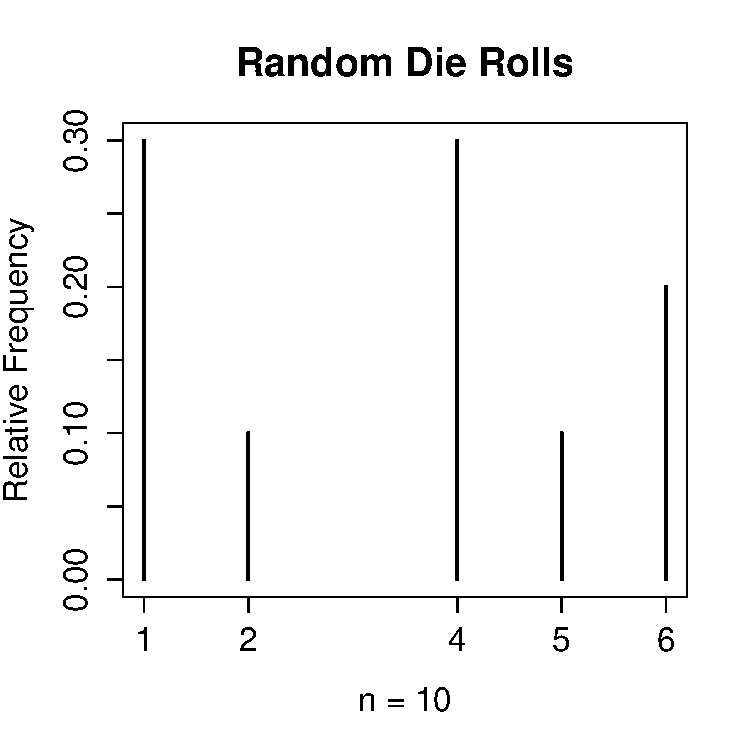
\includegraphics[scale = 0.7]{./images/die1}

\end{frame}
%%%%%%%%%%%%%%%%%%%%%%%%%%%%%%%%%%%%%%%%

\begin{frame}

\centering
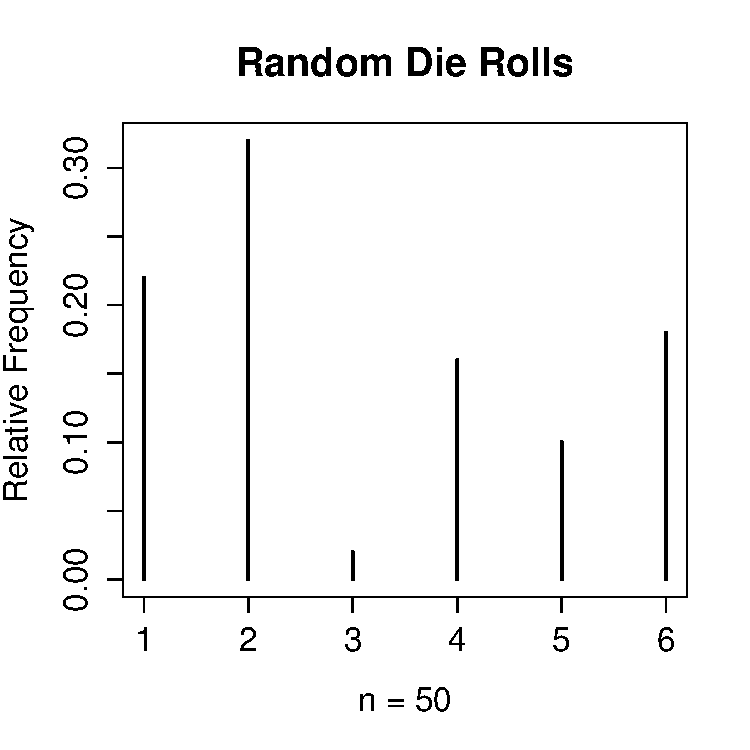
\includegraphics[scale = 0.7]{./images/die2}

\end{frame}
%%%%%%%%%%%%%%%%%%%%%%%%%%%%%%%%%%%%%%%%

\begin{frame}

\centering
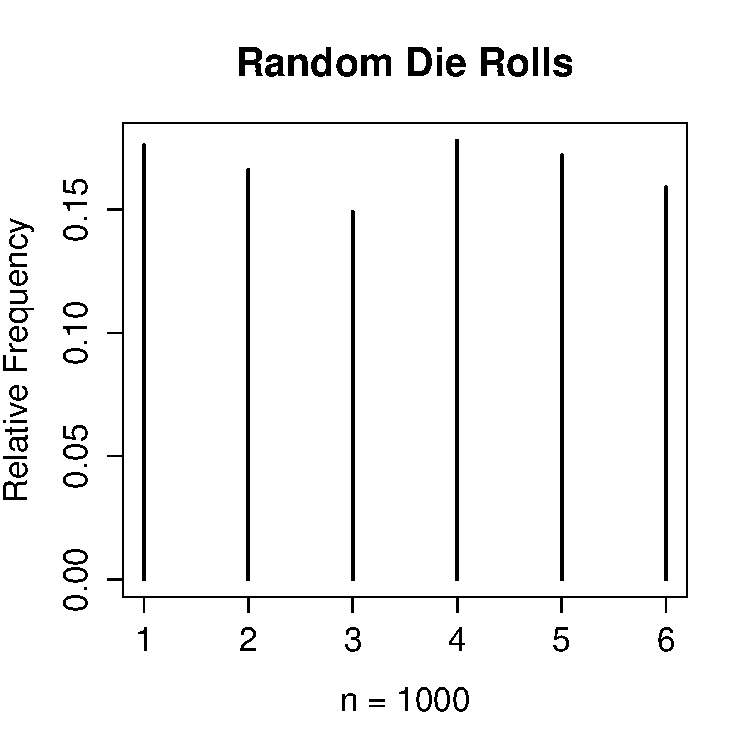
\includegraphics[scale = 0.7]{./images/die3}

\end{frame}
%%%%%%%%%%%%%%%%%%%%%%%%%%%%%%%%%%%%%%%%

\begin{frame}

\centering
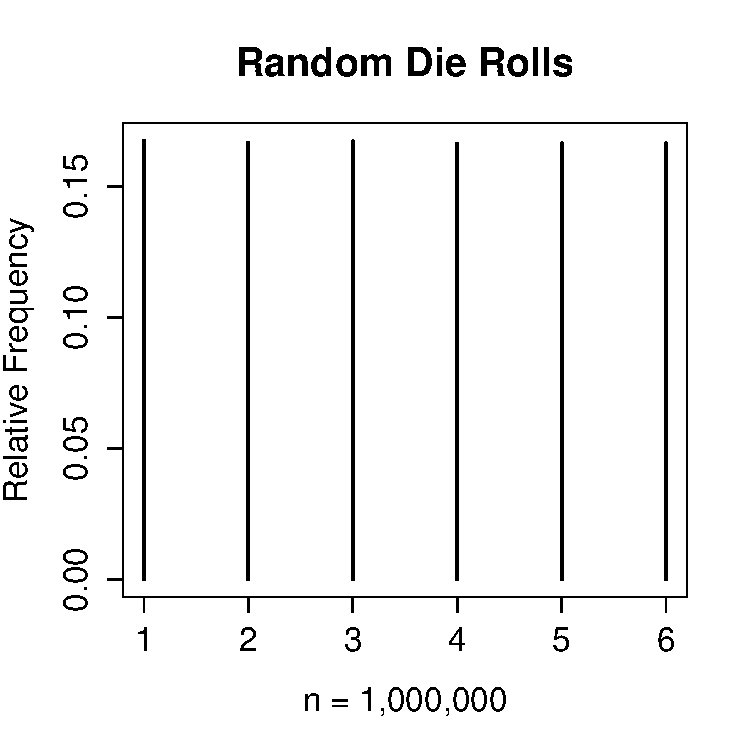
\includegraphics[scale = 0.7]{./images/die4}

\end{frame}
%%%%%%%%%%%%%%%%%%%%%%%%%%%%%%%%%%%%%%%%



\begin{frame}

\frametitle{What do you think of this argument? \hfill 
\includegraphics[scale = 0.05]{./images/clicker}}
\begin{itemize}
	\item The probability of flipping heads is 1/2: if we flip a coin many times, about half of the time it will come up heads.
	\item The last ten throws in a row the coin has come up heads.
	\item The coin is bound to come up tails next time -- it would be very rare to get 11 heads in a row.
\end{itemize}

\begin{enumerate}[(a)]
	\item Agree
	\item Disagree
\end{enumerate}

\end{frame}
%%%%%%%%%%%%%%%%%%%%%%%%%%%%%%%%%%%%%%%%
\begin{frame}

\frametitle{The Gambler's Fallacy}

\begin{alertblock}{Relative frequencies settle down to probabilities, but this does not mean that the trials are dependent.}\end{alertblock}


\begin{block}{Dependent = ``Memory'' of Prev.\ Trials}\end{block}

\begin{block}{Independent = No ``Memory'' of Prev.\ Trials}\end{block}



\end{frame}
%%%%%%%%%%%%%%%%%%%%%%%%%%%%%%%%%%%%%%%%


\begin{frame}
\frametitle{Another Argument \hfill 
\includegraphics[scale = 0.05]{./images/clicker}}
\begin{quote}
Lucie visits Albert. As she enters, he rolls four dice and shouts ``Hooray!'' for he has just rolled four sixes. Lucie: ``I bet you've been rolling the dice for a long time to get that result!'' Now, Lucie may have many reasons for saying this -- perhaps Albert is a lunatic dice-roller. But simply on the evidence that he has just rolled four sixes, is her conclusion reasonable?
\end{quote}

\begin{enumerate}[(a)]
	\item Yes
	\item No
\end{enumerate}

\end{frame}
%%%%%%%%%%%%%%%%%%%%%%%%%%%%%%%%%%%%%%%%
\begin{frame}
\frametitle{The \emph{Inverse} Gambler's Fallacy}

\begin{block}{This is true:}
Albert is more likely to get four sixes if he rolls many times than if he rolls only once.\end{block}
\begin{block}{However:} \emph{Regardless} of how long Albert has been rolling, the probability that he gets four sixes \alert{on the particular roll that Lucie observes} is unchanged. \end{block}
\vspace{2em}
\begin{block}{The outcome of that roll doesn't tell us anything about whether he has rolled the dice before, just like six heads in a row doesn't mean we're ``due'' for a tails.}\end{block}

\end{frame}
%%%%%%%%%%%%%%%%%%%%%%%%%%%%%%%%%%%%%%%%
\begin{frame}
\frametitle{Terminology}
\begin{block}{Random Experiment}
An experiment whose outcomes are random.
\end{block}
\begin{block}{Basic Outcomes}
Possible outcomes (mutually exclusive) of random experiment.
\end{block}
\begin{block}{Sample Space: $S$}
Set of all basic outcomes of a random experiment.
\end{block}

\begin{block}{Event: $E$}
A subset of the Sample Space (i.e.\ a collection of basic outcomes). In set notation we write $E \subseteq S$.
\end{block}

\end{frame}
%%%%%%%%%%%%%%%%%%%%%%%%%%%%%%%%%%%%%%%%
\begin{frame}
\frametitle{Example}
\begin{block}{Random Experiment}
Tossing a pair of dice.
\end{block}
\begin{block}{Basic Outcome}
An ordered pair $(a, b)$ where $a,b \in \{1, 2, 3, 4, 5, 6\}$, e.g.\ $(2,5)$
\end{block}
\begin{block}{Sample Space: $S$}
\emph{All} ordered pairs $(a, b)$ where $a,b \in \{1, 2, 3, 4, 5, 6\}$
\end{block}

\begin{block}{Event: $E = \{\mbox{Sum of two dice is less than 4}\}$}
$\{(1,1), (1,2), (2,1)\}$
\end{block}

\end{frame}
%%%%%%%%%%%%%%%%%%%%%%%%%%%%%%%%%%%%%%%%
\begin{frame}
\frametitle{Visual Representation}
\begin{figure}
\centering
\begin{tikzpicture}[scale = 1.4]
	\draw (0,0) circle [radius = 1];
	\draw (0,1)  node [text=black,above] {$E$};
      \draw (-2,-2) rectangle (3,2);
      \draw (3,2) node [text=black,above] {$S$};
      \draw [fill] (2,0.5) circle [radius=0.03];
      \draw (2,0.5) node [text=black,above] {$O_1$};
      \draw [fill] (0.4,-0.5) circle [radius=0.03];
      \draw (0.4,-0.5) node [text=black,above] {$O_2$};
      \draw [fill] (-0.2,0.3) circle [radius=0.03];
      \draw (-0.2,0.3) node [text=black,above] {$O_3$};
\end{tikzpicture}
\end{figure}
\end{frame}
%%%%%%%%%%%%%%%%%%%%%%%%%%%%%%%%%%%%%%%%

\begin{frame}
\begin{center}
	\Huge Probability is Defined on \emph{Sets}, and Events are Sets
\end{center}
\end{frame}
%%%%%%%%%%%%%%%%%%%%%%%%%%%%%%%%%%%%%%%%
%Some macros for the Venn Diagrams
\def\eventA{(-0.35,0) circle (1.2)}
\def\eventB{(1.35,0) circle (1.2)}
\def\samplespace{(-2,-2) rectangle (3,2)}
%%%%%%%%%%%%%%%%%%%%%%%%%%%%%%%%%%%%%%%%
\begin{frame}
\frametitle{Complement of an Event: $A^c = \mbox{not } A$}

\begin{figure}
\centering
\begin{tikzpicture}[scale = 1.3]

	\fill[blue, fill opacity = 0.5] \samplespace;
	\fill[white, fill opacity = 1] \eventA;
     	\draw \eventA node [above] {$A$};
      \draw \samplespace (3,2) node [text=black,above] {$S$};

\end{tikzpicture}
\caption{The complement $A^c$ of an event $A\subseteq S$ is the collection of all basic outcomes from $S$ not contained in $A$.}
\end{figure}
\end{frame}
%%%%%%%%%%%%%%%%%%%%%%%%%%%%%%%%%%%%%%%%
\begin{frame}
\frametitle{Intersection of Events: $A\cap B = A \mbox{ and } B$}
\begin{figure}
\centering
\begin{tikzpicture}[scale = 1.3]
      \begin{scope}[fill opacity = 0.5]
      \clip \eventA;
      \fill[blue] \eventB;
    \end{scope}
     
     	\draw \eventA node [above] {$A$};
	\draw \eventB node [above] {$B$};
      \draw \samplespace (3,2) node [text=black,above] {$S$};
      
\end{tikzpicture}
\caption{The intersection $A\cap B$ of two events $A,B\subseteq S$ is the collection of all basic outcomes from $S$ contained in both $A$ and $B$}
\end{figure}
\end{frame}
%%%%%%%%%%%%%%%%%%%%%%%%%%%%%%%%%%%%%%%%
\begin{frame}
\frametitle{Union of Events: $A\cup B = A \mbox{ or } B$}
\begin{figure}
\centering
\begin{tikzpicture}[scale = 1.3]

	\begin{scope}[fill opacity = 0.5]
		\fill[blue] \eventA;
		\fill[red] \eventB;
	\end{scope}
	
	\draw \eventA node [above] {$A$};
	\draw \eventB node [above] {$B$};
      \draw \samplespace node [text=black,above] {$S$};
      
\end{tikzpicture}
\caption{The union $A\cup B$ of two events $A,B\subseteq S$ is the collection of all basic outcomes from $S$ contained in $A$, $B$ or both.}
\end{figure}
\end{frame}


%%%%%%%%%%%%%%%%%%%%%%%%%%%%%%%%%%%%%%%%
\begin{frame}
\frametitle{Mutually Exclusive and Collectively Exhaustive}
\begin{block}{Mutually Exclusive Events}
A collection of events $E_1, E_2, E_3, \hdots$ is \emph{\alert{mutually exclusive}} if the intersection $E_i \cap E_j$ of \alert{\emph{any two different events}} is empty.
%(formally $E_i \cap E_j = \emptyset$ for any $i\neq j$).
\end{block}

\begin{block}{Collectively Exhaustive Events}
A collection of events $E_1, E_2, E_3, \hdots$ is \emph{\alert{collectively exhaustive}} if, taken together, they contain \alert{\emph{all of the basic outcomes in $S$}}. Another way of saying this is that the union $E_1 \cup E_2 \cup E_3 \cup \cdots$ is $S$.
\end{block}
\end{frame}
%%%%%%%%%%%%%%%%%%%%%%%%%%%%%%%%%%%%%%%%
\begin{frame}
\frametitle{Implications}
\begin{block}{Mutually Exclusive Events}
  If one of the events occurs, then none of the others did.
\end{block}

\begin{block}{Collectively Exhaustive Events}
  One of these events \emph{must} occur.
\end{block}
\end{frame}
%%%%%%%%%%%%%%%%%%%%%%%%%%%%%%%%%%%%%%%%
%Some macros for collectively exhaustive and mutually exclusive sets
\def\Srect{(-2,-2) rectangle (4,2)}
\def\Arect{(-2,-2) rectangle (0,2)}
\def\Brect{(0,-2) rectangle (2,2)}
\def\Crect{(0,2) rectangle (4,2)}
\def\Devent{(1.6,-0.3) circle (1.3)}
\def\Eevent{(-1,1.2) circle (0.5)}
%%%%%%%%%%%%%%%%%%%%%%%%%%%%%%%%%%%%%%%%
\begin{frame}
\frametitle{Mutually Exclusive but \emph{not Collectively Exhaustive}}
\begin{figure}
\centering
\begin{tikzpicture}[scale = 1.3]
	\draw \Eevent node [above] {$A$};
	\draw \Devent node [above] {$B$};
      \draw \Srect node [above] {$S$};
\end{tikzpicture}
\caption{Although $A$ and $B$ don't overlap, they also don't cover $S$.}
%\caption{Although $A \cap B = \emptyset$, $A \cup B \neq S$}
\end{figure}
\end{frame}

%%%%%%%%%%%%%%%%%%%%%%%%%%%%%%%%%%%%%%%%
\begin{frame}
\frametitle{Collectively Exhaustive but \emph{not Mutually Exclusive}}
\begin{figure}
\centering
\begin{tikzpicture}[scale = 1.3]

	\draw \Arect node [below left] {$A$};
	\draw \Brect node [below left] {$B$};
	\draw \Crect node [below left] {$C$};
	\draw \Devent node [above] {$D$};
      \draw \Srect node [above] {$S$};
\end{tikzpicture}
\caption{Together $A, B, C$ and $D$ cover $S$, but $D$ overlaps with $B$ and $C$.}
%\caption{Although $A \cup B \cup C \cup D = S$, $B \cap D \neq \emptyset$ and $C \cap D \neq \emptyset$.}
\end{figure}
\end{frame}

%%%%%%%%%%%%%%%%%%%%%%%%%%%%%%%%%%%%%%%%
\begin{frame}
\frametitle{Collectively Exhaustive \emph{and} Mutually Exclusive}
\begin{figure}
\centering
\begin{tikzpicture}[scale = 1.3]

	\draw \Arect node [below left] {$A$};
	\draw \Brect node [below left] {$B$};
	\draw \Crect node [below left] {$C$};
      \draw \Srect node [above] {$S$};
\end{tikzpicture}
\caption{$A$, $B$, and $C$ cover $S$ and don't overlap.}
%\caption{$A \cup B \cup C = S$, and $A \cap B = B\cap C = A \cap C = \emptyset$.}
\end{figure}
\end{frame}

%%%%%%%%%%%%%%%%%%%%%%%%%%%%%%%%%%%%%%%%

\begin{frame}
\frametitle{Axioms of Probability}
We assign every event $A$ in the sample space $S$ a real number $P(A)$ called the \alert{probability of $A$} such that: 
\vspace{1em}
\begin{description}
	\item[Axiom 1] $0 \leq P(A) \leq 1$
	\item[Axiom 2] $P(S)=1$
	\item[Axiom 3] If $A_1, A_2, A_3, \hdots$ are mutually exclusive events, then $P(A_1\cup A_2 \cup A_3 \cup \cdots) = P(A_1) + P(A_2) + P(A_3) + \hdots$
\end{description}

\end{frame}
%%%%%%%%%%%%%%%%%%%%%%%%%%%%%%%%%%%%%%%%

\begin{frame}

\frametitle{``Classical'' Probability}

When all of the basic outcomes are equally likely, calculating the probability of an event is simply a matter of counting -- count up all the basic outcomes that make up the event, and divide by the total number of basic outcomes.

\end{frame}
%%%%%%%%%%%%%%%%%%%%%%%%%%%%%%%%%%%%%%%%
\begin{frame}
\frametitle{Recall from High School Math:}

\begin{block}{Multiplication Rule for Counting}
$n_1$ ways to make first decision, $n_2$ ways to make second, $\hdots, n_k$ ways to make kth $\Rightarrow n_1 \times n_2 \times \cdots \times n_k$ total ways to decide. \end{block}
\begin{block}{Corollary -- Number of Possible Orderings}
$k \times(k-1)\times (k-2) \times \cdots\times  2 \times 1 = k!$
\end{block}

\begin{block}{Permutations -- Order $n$ people in $k$ slots}
$P_k^n = \frac{n!}{(n-k)!}$ \hfill \alert{(Order Matters)}\end{block}

\begin{block}{Combinations -- Choose committee of $k$ from group of $n$}
${n \choose k} = \frac{n!}{k! (n-k)!}$, where $0! = 1$\hfill \alert{(Order Doesn't Matter)}\end{block}

\end{frame}
%%%%%%%%%%%%%%%%%%%%%%%%%%%%%%%%%%%%%%%%

\begin{frame}

\frametitle{Poker -- Deal 5 Cards, Order Doesn't Matter}

\begin{block}{Basic Outcomes}
\vspace{0.3em} 
$\displaystyle{52 \choose 5}$ possible hands
\end{block}
\begin{block}{How Many Hands have Four Aces? \hfill 
\includegraphics[scale = 0.05]{./images/clicker} } \pause
\alert{48 (\# of ways to choose the single card that is not an ace)}
\end{block}

\begin{block}{Probability of Getting Four Aces}
\vspace{0.3em} 
$48/\displaystyle{52 \choose 5} \approx 0.00002$
\end{block}


\end{frame}
%%%%%%%%%%%%%%%%%%%%%%%%%%%%%%%%%%%%%%%%
\begin{frame}
\frametitle{Poker -- Deal 5 Cards, Order Doesn't Matter}
\begin{block}{What is the probability of getting 4 of a kind?}
	\begin{itemize}
		\item 13 ways to choose \emph{which} card we have four of
		\item 48 ways to choose the last card in the hand 
		\item $13 \times 48 = \alert{624}$ 
	\end{itemize}
\end{block}
\vspace{0.3em} 
$624/\displaystyle{52 \choose 5} \approx 0.00024$

\end{frame}
%%%%%%%%%%%%%%%%%%%%%%%%%%%%%%%%%%%%%%%%
\begin{frame}
\frametitle{A Fairly Ridiculous Example \hfill 
\includegraphics[scale = 0.05]{./images/clicker}}

Roger Federer and Novak Djokovic have agreed to play in a tennis tournament against six Penn professors. Each player in the tournament is randomly allocated to one of the eight rungs in the ladder (next slide). Federer always beats Djokovic and, naturally, either of the two pros always beats any of the professors. What is the probability that Djokovic gets second place in the tournament? 



\end{frame}
%%%%%%%%%%%%%%%%%%%%%%%%%%%%%%%%%%%%%%%%

\begin{frame}
\begin{figure}
\centering
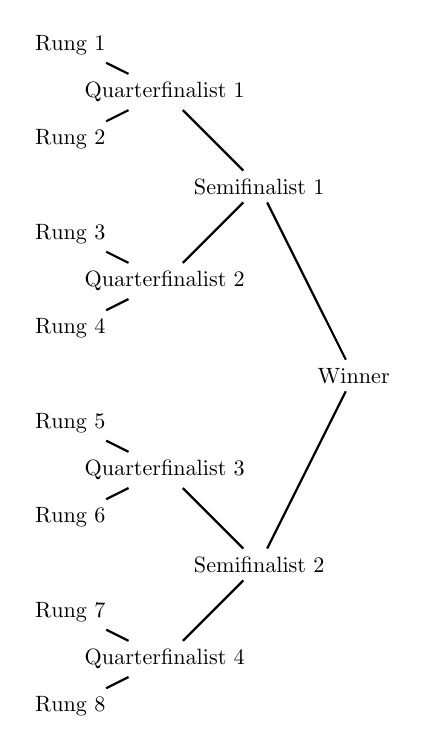
\begin{tikzpicture}[thick,scale=0.8, every node/.style={transform shape},grow'=left]
\node {Winner} 
  [sibling distance=6cm]
  child {node {Semifinalist 2}
  [sibling distance=3cm]
    child {node {Quarterfinalist 4}
    	    [sibling distance=1.5cm]
    	child {node {Rung 8}}
    	child {node {Rung 7}}
    }
    child {node {Quarterfinalist 3}
        [sibling distance=1.5cm]
    	child {node {Rung 6}}
    	child {node {Rung 5}}
    }
  }
  child {node {Semifinalist 1}
  [sibling distance=3cm]
    child {node {Quarterfinalist 2}
    [sibling distance=1.5cm]
    	child {node {Rung 4}}
    	child {node {Rung 3}}
    }
    child {node {Quarterfinalist 1}
        [sibling distance=1.5cm]
    	child {node {Rung 2}}
    	child {node {Rung 1}}
    }
  };
\end{tikzpicture}
\raisebox{4.4em}{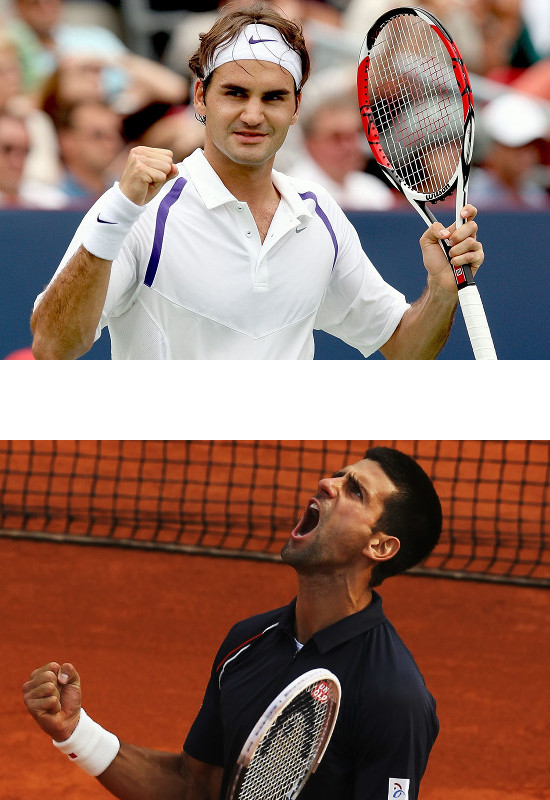
\includegraphics[scale=0.8]{./images/tennisplayers}} 
\end{figure}


\end{frame}

%%%%%%%%%%%%%%%%%%%%%%%%%%%%%%%%%%%%%%%%
\begin{frame}
  \frametitle{Solution: Order Matters!}
  \begin{block}{Denominator}
	$8!$ basic outcomes -- ways to arrange players on tournament ladder.
  \end{block}
  \begin{block}{Numerator}
   Sequence of three decisions:
   \begin{enumerate}
    \item Which rung to put Federer on? (8 possibilities)
    \item Which rung to put Djokovic on? 
      \begin{itemize}
        \item For any given rung that Federer is on, only 4 rungs prevent Djokovic from meeting him until the final.
      \end{itemize}
    \item How to arrange the professors? ($6!$ ways)
   \end{enumerate}
  \end{block}
\alert{$$\frac{8 \times 4 \times 6!}{8!} = \frac{8\times 4}{7\times 8} = 4/7 \approx 0.57$$}

\end{frame}
%%%%%%%%%%%%%%%%%%%%%%%%%%%%%%%%%%%%%%%%
\begin{frame}

\centering \Huge Even if the basic outcomes are equally likely, the events of interest may not be...


\end{frame}
%%%%%%%%%%%%%%%%%%%%%%%%%%%%%%%%%%%%%%%%
\begin{frame}
\frametitle{``Odd Question'' \# 4}
To throw a total of 7 with a pair of dice, you have to get a 1 and a 6, or a 2 and a 5, or a 3 and a 4.
To throw a total of 6 with a pair of dice, you have to get a 1 and a 5, or a 2 and a 4, or a 3 and another 3.
	\vspace{1em}
	With two fair dice, you would expect:
		\begin{enumerate}[(a)]
			\item To throw 7 more frequently than 6.
			\item To throw six more frequently than 7.
			\item To throw 6 and 7 equally often.
		\end{enumerate}
\end{frame}
%%%%%%%%%%%%%%%%%%%%%%%%%%%%%%%%%%%%%%%%
\begin{frame}
\frametitle{Basic Outcomes Equally Likely, Events of Interest Aren't}

\begin{table}
	\begin{tabular}{|lr|cccccc|}
	\hline
	&&\multicolumn{6}{|c|}{Second Die}\\
	&&1&2&3&4&5&6\\
	\hline
	&1&2&3&4&5&\alert{6}&\textcolor{blue}{7}\\
	&2&3&4&5&\alert{6}&\textcolor{blue}{7}&8\\
	First&3&4&5&\alert{6}&\textcolor{blue}{7}&8&9\\
	Die&4&5&\alert{6}&\textcolor{blue}{7}&8&9&10\\
	&5&\alert{6}&\textcolor{blue}{7}&8&9&10&11\\
	&6&\textcolor{blue}{7}&8&9&10&11&12\\
	\hline
	\end{tabular}
	\caption{There are 36 equally likely basic outcomes, of which 5 correspond to a sum of six and 6 correspond to a sum of  seven.}
\end{table}
	\alert{$P(7) = 6/36 = 1/6$}\\
	\alert{$P(6) = 5/36$}
\end{frame}

%%%%%%%%%%%%%%%%%%%%%%%%%%%%%%%%%%%%%%%%
\end{document}
